\section{Pipelining}

\begin{defi}{Pipelining}
    % TODO: https://de.wikipedia.org/wiki/Pipeline_(Prozessor) (Quelle)
    Die \emph{Pipeline} (auch Befehls-Pipeline oder Prozessor-Pipeline) bezeichnet bei Mikroprozessoren eine Art \enquote{Fließband}, mit dem die Abarbeitung der Maschinenbefehle in Teilaufgaben zerlegt wird, die für mehrere Befehle parallel durchgeführt werden.
    
    Dieses Prinzip, oft auch kurz \emph{Pipelining} genannt, stellt eine weit verbreitete Mikroarchitektur heutiger Prozessoren dar.
    
    Statt eines gesamten Befehls wird während eines Taktzyklus des Prozessors nur jeweils eine Teilaufgabe abgearbeitet, allerdings werden die verschiedenen Teilaufgaben mehrerer Befehle dabei gleichzeitig bearbeitet.
    Da diese Teilaufgaben einfacher (und somit schneller) sind als die Abarbeitung des gesamten Befehls am Stück, kann durch Pipelining die Effizienz der Taktfrequenz des Mikroprozessors gesteigert werden.
    Insgesamt benötigt ein einzelner Befehl nun mehrere Takte zur Ausführung, da aber durch die quasi parallele Bearbeitung mehrerer Befehle in jedem Zyklus ein Befehl \enquote{fertiggestellt} wird, wird der Gesamtdurchsatz durch dieses Verfahren erhöht.
    
    Die einzelnen Teilaufgaben einer Pipeline nennt man Pipeline-Stufen, Pipeline-Stages oder auch Pipeline-Segmente.
    Diese Stufen werden durch getaktete Pipeline-Register getrennt.
    
    Neben einer Befehls-Pipeline kommen in modernen Systemen verschiedene weitere Pipelines zum Einsatz, beispielsweise eine Arithmetik-Pipeline in der Gleitkommaeinheit.
\end{defi}

\begin{example}[Pipelining]{RISC vs. CISC}
    TODO: Grafik
\end{example}

\subsection{Pipelining auf Instruktionsebene (ILP)}

\begin{defi}[Pipelining]{Funktionseinheiten}
    Eine fünfstufige Pipeline, z. B. beim \emph{MIPS-Prozessor} (\emph{Microprocessor without Interlocked Pipelined Stages}, eine RISC-Befehlssatzarchitektur), wird aus folgenden Funktionseinheiten gebildet:
    \begin{itemize}
        \item \emph{IF}: Instruction Fetch
        \item \emph{ID}: Instruction Decode
        \item \emph{EX}: Execution
        \item \emph{MEM}: Memory Access
        \item \emph{WB}: Write Back
    \end{itemize}
    
    % TODO: https://commons.wikimedia.org/wiki/File:5_Stage_Pipeline.svg (Quelle)
    \centering
    % 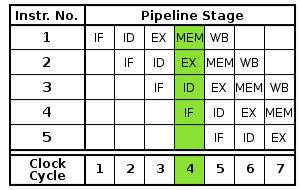
\includegraphics[width=0.5\linewidth]{images/5_stage_pipeline.png}
    \begin{tabular}{|c|c|c|c|c|c|c|c|}
        \toprule
        Instr. No.  & \multicolumn{7}{c|}{Pipeline Stage}                                   \\
        \toprule
        1           & IF                                  & ID & EX & MEM & WB  &     &     \\
        \midrule
        2           &                                     & IF & ID & EX  & MEM & WB  &     \\
        \midrule
        3           &                                     &    & IF & ID  & EX  & MEM &     \\
        \midrule
        4           &                                     &    &    & IF  & ID  & EX  & MEM \\
        \midrule
        5           &                                     &    &    &     & IF  & ID  & EX  \\
        \midrule
        \midrule
        Clock Cycle & 1                                   & 2  & 3  & 4   & 5   & 6   & 7   \\
        \bottomrule
    \end{tabular}
\end{defi}

\begin{defi}[Pipelining]{Taktung}
    % TODO: https://de.wikipedia.org/wiki/Pipeline_(Prozessor)#Taktung (Quelle)
    Je einfacher eine einzelne Stufe aufgebaut ist, desto höher ist die \emph{Frequenz}, mit der sie betrieben werden kann.
    In einer modernen CPU mit einem Kerntakt im Gigahertz-Bereich kann die Befehlspipeline über 30 Stufen lang sein.
    Der \emph{Kerntakt} ist die Zeit, die ein Befehl braucht, um eine Stufe der Pipeline zu durchwandern.
    
    In einer $k$-stufigen Pipeline wird ein Befehl also in $k$ Takten von $k$ Stufen bearbeitet.
    Da in jedem Takt ein neuer Befehl geladen wird, verlässt im Idealfall auch ein Befehl pro Takt die Pipeline.
    
    Der \emph{Takt} wird durch die Zykluszeit der Pipeline bestimmt und berechnet sich aus dem Maximum $\tau_{m}$ aller Stufenverzögerungen $\tau_{i}$ und einem Zusatzaufwand $d$, welcher durch die Zwischenspeicherung der Ergebnisse in Pipeline-Registern verursacht wird.
    
    Die Zykluszeit $\tau$ ist dann definiert durch:
    \[
        \tau = \max_i (\tau_i) + d = \tau_m + d
    \]
\end{defi}

\begin{defi}[Pipelining]{Durchsatz}
    % TODO: https://de.wikipedia.org/wiki/Pipeline_(Prozessor)#Taktung (Quelle)
    Durch das Pipelining wird der \emph{Gesamtdurchsatz} gegenüber Befehlsabarbeitung ohne Pipelining erhöht.
    Die Gesamtzeit für die Pipeline-Verarbeitung mit $k$ Stufen und $n$ Befehlen bei einer Zykluszeit $\tau$ ergibt sich aus:
    \[
        T_k = (k + n - 1) \cdot \tau
    \]
    Erklärung: Anfangs ist die Pipeline leer und wird in $k \cdot \tau$ Schritten gefüllt.
    Nach jeder Stufe wird ein neuer Befehl in die Pipeline geladen, und ein anderer Befehl wird fertiggestellt.
    Die restlichen Befehle werden daher in $(n-1)\cdot \tau$ Schritten fertiggestellt.
\end{defi}

\begin{defi}[Pipelining]{Speedup}
    % TODO: https://de.wikipedia.org/wiki/Pipeline_(Prozessor)#Taktung (Quelle)
    Der bestmögliche \emph{Speedup} beim Pipelining entspricht der Anzahl der Pipeline-Stufen.
    Er wird reduziert durch unausgewogene Ausführungslängen.
    Die Geschwindigkeit der Pipeline ist also direkt beschränkt durch die langsamste Pipeline-Stufe.
    
    Eine effiziente Pipeline-Nutzung setzt voraus, dass eine möglichst hohe Anzahl von Aufträgen (Prozesse) verarbeitet wird.
    Bei nur einem Auftrag entartet die Pipeline zu einer reinen sequentiellen Verarbeitung.
    
    Bildet man nun den Quotienten aus der Gesamtlaufzeit für Befehlsabarbeitung mit und ohne Pipelining, so erhält man den Speedup bei $k$ Stufen und $n$ Befehlen bei einer Zykluszeit $\tau$:
    \[
        S_k = \frac{n \cdot (k \cdot \tau)}{(k + n - 1) \cdot \tau} = \frac{n \cdot k}{k + n - 1}
    \]
\end{defi}

\begin{defi}{Superskalarität}
    Unter \emph{Superskalarität} versteht man die Fähigkeit eines Prozessors, zwei oder mehr skalare Befehle eines Befehlsstroms gleichzeitig mit Hilfe von mehreren parallel arbeitenden Funktionseinheiten auszuführen.
    
    Es handelt sich dabei um eine Nebenläufigkeit bei der Ausführung einzelner Maschinenanweisungen.
    Dazu müssen die parallel abgearbeiten Befehle voneinander unabhängig sein und der Prozessor muss mindestens zwei parallel betreibbare Ausführungseinheiten besitzen.
    
    Superskalarität ermöglicht es, mehr als eine Maschinenanweisung pro Takt zu bearbeiten, während Pipelining die maximal mögliche Taktfrequenz erhöht.
\end{defi}

\begin{defi}{Pipeline-Hazard}
    % TODO: https://de.wikipedia.org/wiki/Pipeline-Hazard (Quelle)
    Alle modernen Prozessoren sind in Pipeline-Architektur ausgeführt:
    Die einzelnen Instruktionen durchlaufen eine mehrstufige Pipeline, in der sie bei jedem Taktzyklus die nächste Stufe erreichen.
    
    Jeder Teilschritt benötigt gewisse Ressourcen des Prozessors (z. B. Datenwege und Rechenwerke) und möglicherweise Ergebnisse einer vorhergegangenen Instruktion.
    Falls eine dieser Ressourcen von einer anderen Instruktion blockiert ist oder Ergebnisse noch nicht zur Verfügung stehen, muss diese Instruktion und alle in der Pipeline folgenden vorübergehend angehalten (\enquote{stalled}) werden.
    
    Die Risiken, den Strom der gleichmäßigen Abarbeitung abreißen zu lassen, nennt man \emph{Pipeline-Hazards}.
\end{defi}

\begin{defi}[Pipeline-Hazard]{Structural Hazards}
    % TODO: https://de.wikipedia.org/wiki/Pipeline-Hazard (Quelle)
    \emph{Structural Hazards} bzw. \emph{Strukturkonflikte} treten auf, wenn Ressourcenkonflikte innerhalb von Befehlen in der Pipeline vorhanden sind, z. B. ein synchroner Zugriff auf einen Registerspeicher mit nur einem Eingang.
    
    Das Beispiel zeigt, dass es sinnvoll ist, voneinander abhängige Befehle möglichst nicht direkt hintereinander auszuführen.
    Moderne Prozessoren können deshalb durch Out-of-Order Execution oder hardwareseitiges Multithreading in vielen Fällen Hazards und Ressourcenkonflikte vermeiden.
\end{defi}

\begin{defi}[Pipeline-Hazard]{Data Hazards}
    % TODO: https://de.wikipedia.org/wiki/Pipeline-Hazard (Quelle)
    \emph{Data Hazards} bzw. \emph{Datenkonflike} ergeben sich aus Datenabhängigkeiten zwischen Befehlen im Programm.
\end{defi}

\begin{defi}{Schleifenparallelisierung}
    % TODO: https://en.wikipedia.org/wiki/Loop_dependence_analysis vlt hilfreich (Quelle)
    TODO
\end{defi}

\begin{defi}{Abhängigkeitsgraph}
    % TODO: https://en.wikipedia.org/wiki/Loop_dependence_analysis vlt hilfreich (Quelle)
    TODO
\end{defi}

\begin{defi}[Pipeline-Hazard]{Control Hazards}
    % TODO: https://de.wikipedia.org/wiki/Pipeline-Hazard (Quelle)
    \emph{Control Hazards} bzw. \emph{Steuerkonflikte} treten bei Instruktionen auf, die den Befehlszähler verändern, z. B. bei bedingten Sprungbefehlen (Branching).
\end{defi}

\begin{defi}{Sprungvorhersage}
    % TODO: https://de.wikipedia.org/wiki/Pipeline-Hazard (Quelle)
    % TODO: https://de.wikipedia.org/wiki/Sprungvorhersage (Quelle)
    Mit der \emph{Predication}-Methode bzw. \emph{Sprungvorhersage} können bestimmte Control Hazards (Branches) aufgelöst werden.
    
    Sie besteht aus den Schritten:
    \begin{enumerate}
        \item Vorhersage, ob ein bedingter Sprung ausgeführt wird
        \item Zieladresse eines Sprunges ermitteln
    \end{enumerate}
\end{defi}

\begin{defi}[Befehlssatzarchitektur]{VLIW}
    % TODO: https://de.wikipedia.org/wiki/Very_Long_Instruction_Word (Quelle)
    \emph{Very Long Instruction Word} (\emph{Very Long Instruction Word}) bezeichnet eine Eigenschaft einer Befehlssatzarchitektur einer Familie von Mikroprozessoren.
    Ziel ist die Beschleunigung der Abarbeitung von sequentiellen Programmen durch Ausnutzung von Parallelität auf Befehlsebene.
    
    Im Gegensatz zu superskalaren Prozessoren werden bei VLIW die Befehle nicht dynamisch zur Laufzeit vom Prozessor den einzelnen Funktionseinheiten zugewiesen, sondern der Compiler gruppiert parallel ausführbare Befehle.
    
    VLIW schließt die Verwendung einer Pipeline-Architektur nicht aus.
    
    TODO: Grafik
\end{defi}

\begin{defi}[Befehlssatzarchitektur]{Explicitly Parallel Instruction Computing (EPIC)}
    Von HP und Intel wurde 1998/99 die Prozessorarchitektur EPIC entworfen und mit dem Intel Itanium ein erster Prozessor realisiert. 
    Die Intel-Version der Architektur wird IA-64 (64 bit) genannt.
    
    EPIC ist die moderne Weiterentwicklung des Konzepts des VLIW.
    
    Hierbei versucht der Compiler, möglichst viele voneinander unabhängige Instruktionen in einer Sequenz zusammenzustellen. 
    Er kann dabei durch Umstellen der Befehle die Reihenfolge innerhalb der Sequenz verändern. Dies darf aber nicht zu anderen Ergebnissen führen!
    Eine solche Sequenz nennt Intel ein \enquote{bundle}.
    
    Das \emph{Explicitly Parallel Instruction Computing} (\emph{EPIC}) bezeichnet ein Programmierparadigma einer Befehlssatzarchitektur.
    Bei der Programmierung von EPIC-CPUs wird die Parallelisierung der Befehle eines Instruktionsstromes explizit vorgenommen.
    
    Die Instruction Set Architecture (ISA) hat Eigenschaften, die die explizite Parallelisierung unterstützen, während eine herkömmliche ISA von einer sequentiellen Abarbeitung der Befehle ausgeht.
    
    Ein Programm, das in einer Nicht-EPIC-Maschinensprache vorliegt, kann auch parallelisiert werden, aber es ist bei der Ausführung eine komplexe Logik notwendig, um parallel ausführbare Instruktionen zu identifizieren, da das Befehlsformat keine Aussagen über parallelisierbare Instruktionen macht.
    
    Eine EPIC-CPU arbeitet nach dem Prinzip der in-order Execution, im Gegensatz zur out-of-order execution der superskalaren CPUs.
\end{defi}

\begin{defi}{Speculative Execution}
    Bei \emph{Speculative Execution} werden untätige Prozessor-Ressourcen verwendet, um für einen potentiellen zukünftigen Stand des Programmflusses Berechnungen vorauszuführen und Ergebnisse bereitzuhalten.
    
    Hier werden in Phasen, in denen der Prozessor nicht voll ausgelastet ist, die folgenden Programmschritte (in der Programmflusszukunft) auf ihre Ausführbarkeit untersucht mit dem Ziel, den wahrscheinlichsten Weg des Programmflusses zu finden.
    Der wahrscheinlichste Ausführungsweg wird verfolgt, und die Ergebnisse werden als \enquote{spekulative Ergebnisse} zwischengespeichert.
    Wenn das Programm an der Stelle angekommen ist, an dem es die Ergebnisse benötigt, stehen sie schon zur Verfügung und es muss nicht auf eine möglicherweise langwierige Berechnung gewartet werden.
    Die zwischengespeicherten Ergebnisse werden ausgelesen und das Passende ausgeführt, die Anderen werden verworfen.
    
    Durch dieses \enquote{Vorausschauen} des Prozessors wird dessen Leistungsfähigkeit auch in Phasen geringerer Auslastung genutzt, um ihn bei hoher Auslastung später zu entlasten.
\end{defi}

\begin{defi}[Speculative Execution]{Control Speculation}
    % http://www.cs.cmu.edu/afs/cs/academic/class/15740-f03/www/lectures/valuepred-slides.pdf
    TODO: Sinnvolle Definition
\end{defi}

\begin{defi}[Speculative Execution]{Data Speculation}
    % http://www.cs.cmu.edu/afs/cs/academic/class/15740-f03/www/lectures/valuepred-slides.pdf
    TODO: Sinnvolle Definition
\end{defi}

\begin{defi}{Attached-Processor-Systeme}
    Eine zusätzliche Einheit,
    die in einer Multiprozessor-Umgebung an die primäre CPU angeschlossen ist.
    Sie arbeitet als Erweiterung der primären CPU und
    nutzt die Systemsoftware und Peripheriegeräte gemeinsam.
\end{defi}